% \chapter{Phương pháp xử lý ngôn ngữ tự nhiên}
\section{Giới thiệu về xử lý ngôn ngữ tự nhiên}
\label{sec:introduction_nlp}
Xử lý ngôn ngữ tự nhiên (Natural Language Processing - NLP) là một nhánh của trí tuệ nhân tạo tập trung vào các ứng dụng trên ngôn ngữ của con người. Trong trí tuệ nhân tạo thì xử lý ngôn ngữ tự nhiên là một trong những phần khó nhất vì nó liên quan đến việc phải hiểu ý nghĩa ngôn ngữ-công cụ hoàn hảo nhất của tư duy và giao tiếp.

NLP có thể được hiểu ngắn gọn là khả năng xử lý ngôn ngữ của con người (thường được khái quát là tự nhiên), vì ngôn ngữ con người được sử dụng trong hình ảnh, viết, nói,... Từ \emph{xử lý} (process) trong từ "Xử lý ngôn ngữ tự nhiên" có nghĩa là: "Thay đổi một cái gì đó thành một thứ khác". Trong trường hợp này có nghĩa là "Lấy từ ngôn ngữ của con người và biến thành các biểu diễn mà máy tính có thể hiểu và xử lý". Ví dụ: Những từ mà bạn đang đọc và viết dưới dạng ngôn ngữ tự nhiên (tiếng Việt bằng các ký tự latin) và được lưu trong ngôn ngữ máy tính (dạng nhị phân gồm các chuỗi số gồm 0 và 1). Tuy nhiên, NLP không phải chỉ là chuyển các ký tự trong bảng chữ cái thành các bit. Nó liên quan nhiều hơn đến việc làm cho máy tính có thể hiểu, xử lý một cách tự động (hoặc làm một số tác vụ liên quan đến ngôn ngữ) dựa trên cách ngôn ngữ của con người được biểu diễn và tổ chức [\ref{refer:7}].

NLP thường liên quan đến những việc sau:
\begin{itemize}
    \item Những từ nào trong cụm từ là danh từ?
    \item Danh từ nào trong cụm từ đóng vai trò chính trong cụm từ gốc?
    \item Cụm từ này thể hiện cảm xúc gì?
    \item Từ này trong ngữ cảnh này có thể hiểu là gì?
    \item và nhiều tác vụ khác
\end{itemize}

Các ứng dụng sử dụng NLP gồm có:
\begin{itemize}
    \item \emph{Phân tích cảm xúc} (Sentiment Analysis - SA): Những đoạn văn bản có thể mang trong nó các sắc thái hoàn cảnh và có thể rất phức tạp. Ví dụ như bạn của bạn đang buồn hay tức giận, bạn sẽ có những cách hỏi chuyện khác nhau. Hay việc sử dụng từ hoặc dấu câu theo ngữ cảnh khác nhau sẽ dẫn đến những cách hiểu khác nhau. Cảm xúc có thể nhận ra từ sự kết hợp của giọng điệu, sự lựa chọn từ ngữ và phong cách viết. SA được dùng để hiễu sâu sắc hơn về ngữ cảnh của văn bản. Ví dụ như: việc đánh giá cảm xúc thích hay không thích về một sản phẩm tiểu dùng dựa trên hàng ngàn bình luận trên mạng xã hội có thể giúp cải thiện chiến dịch truyền thông của sản phẩm đó. Hay bạn có thể đánh giá dự báo thị trường chứng khoáng thông qua đánh giá mức độ lạc quan của hàng ngàn người trên một diễn đàn tài chính để giúp hỗ trợ đầu tự. Hoặc những chính trị gia có thể đánh giá phản ứng của hàng trăm ngàn người với mỗi nội dung của các chính trị gia đưa trên Twitter, Facebook.
    \item \emph{Phân loại văn bản} (Text Classification - TC): Đây có thể được coi là một trong những ứng dụng phổ biến nhất của NLP. Trong TC, các từ (nghĩa, mối quan hệ các từ, ngữ cảnh) được sử dụng như là các đặc tính để dùng cho các thuật toán xác định văn bản thuộc về lớp X, Y hay Z. Ví dụ: Google sử dụng giải thuật TC để phân loại thư điện tử gửi đến có phải là thư rác hay không.
    \item \emph{Nhận diện chủ thể} (Entity Recognition - ER): Xác định và nhận diện thông tin chính (chủ thể) trong văn bản. Một chủ thể có thể là một từ hoặc một chuỗi từ mà liên tục đề cập đến cùng một thứ. Mỗi chủ thể sẽ được xác định và đưa vào các thể loại định trước. Ví dụ như xác định từ "Microsoft" trong văn bản và phân loại nó thành mục "Công ty"[\ref{refer:8}].
    \item \emph{Nhận diện chủ đề} (Topic Modeling - TM): Trong NLP, thuật ngữ "chủ đề" có nghĩa là tập các từ ngữ "đi cùng với nhau". Những từ ngữ này ta sẽ gợi nhớ ra khi nghĩ đến chủ đề cụ thể. Ví dụ như chủ đề "thể thao" thì sẽ gợi nhớ ra các từ như: bóng đá, sân vận động, chạy bộ, bơi lội,... [\ref{refer:9}].
    \item \emph{Dịch máy} (Machine Translation): NLP có thể giúp phiên dịch tự động văn bản từ ngôn ngữ này sang một ngôn ngữ khác. Có nhiều thách thức đối với dịch máy bao gồm như: sự đa dạng về ngôn ngữ, bảng chữ cái và ngữ pháp, khó khăn khi xác định việc phiên dịch có chính xác hay không [\ref{refer:10}].
    % \item \emph{Nhận diện giọng nói} (Speech Recognition)
    \item \emph{Trả lời tin nhắn tự động} (Chatbot): với sự hỗ trợ của NLP, chatbot có thể dễ dàng hiểu được câu hỏi của khách hàng với những từ ngữ tự nhiên hơn mà khong cần sự hỗ trợ từ con người.
    \item \emph{Tự động tóm tắt văn bản (Automatic Summarization)}: Tóm tắt văn bản là nhiệm vụ cô đọng một đoạn văn bản thành phiên bản ngắn hơn, giảm kích thước của văn bản ban đầu đồng thời bảo tồn các yếu tố thông tin chính và ý nghĩa của nội dung. Vì tóm tắt văn bản thủ công là một công việc tốn kém thời gian và thường tốn nhiều công sức, việc tự động hóa tác vụ này đang ngày càng phổ biến và do đó tạo thành động lực mạnh mẽ cho nghiên cứu học thuật.
    \item và các ứng dụng khác.
\end{itemize}

\subsection{Mô hình xử lý ngôn ngữ tự nhiên cổ điển}
\label{sec:classic_nlp}
Theo phương pháp cổ điển, các tác vụ xử lý ngôn ngữ tự nhiên gồm có 2 bước chính như sau:
\begin{itemize}
    \item Tiền xử lý (Pre-processing)
    \item Mô hình hóa (Modeling)
\end{itemize}

Hình \ref{fig:pipeline-nlp-classic} mô tả mô hình xử lý ngôn ngữ tự nhiên cổ điển. Thông qua 2 bước pre-processcing và modeling ta sẽ nhận được output mong muốn như là: Phân tích cảm xúc, Phân loại văn bản,...

\begin{figure}[h!]
\begin{center}
	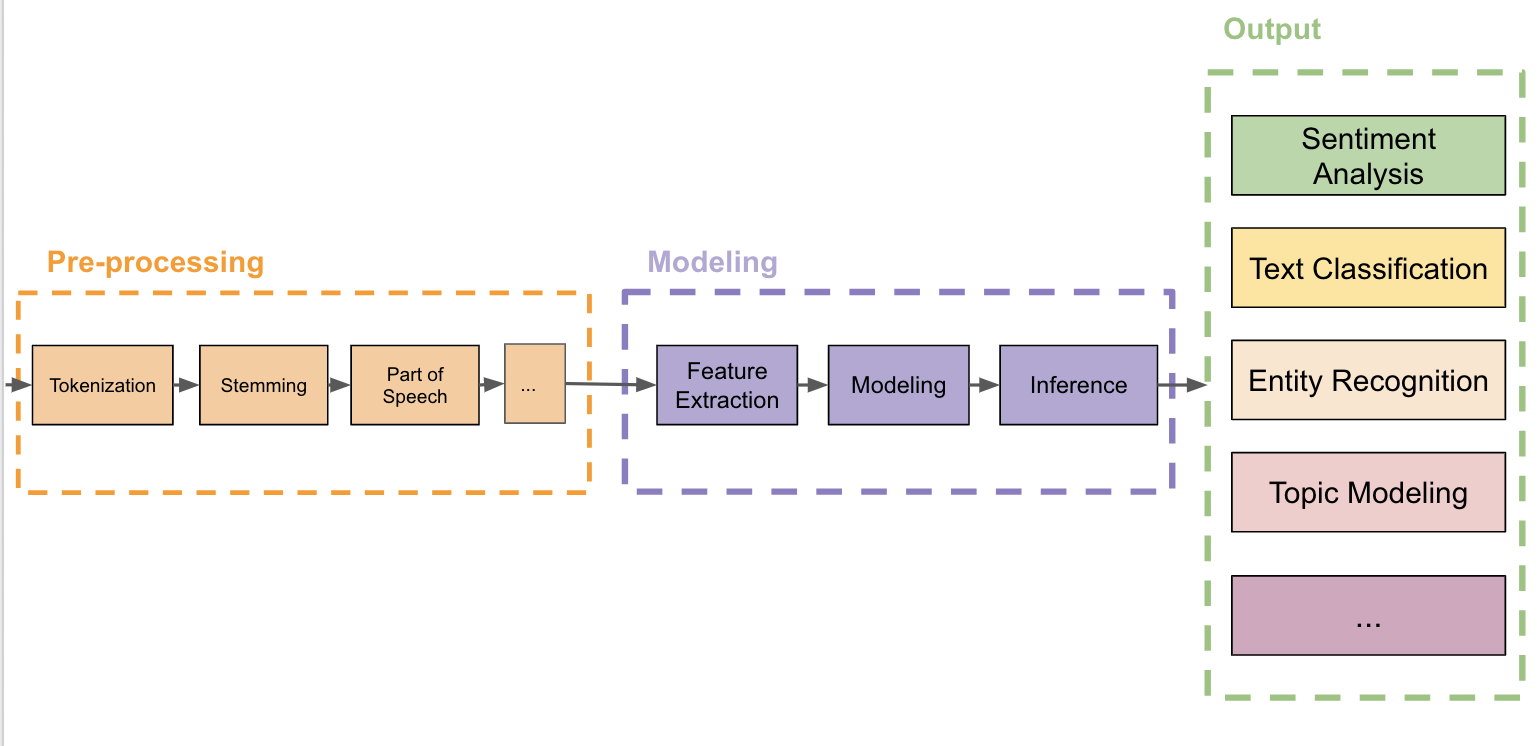
\includegraphics[width=1.0\textwidth]{books/artificial-neural-network/chapter04/figure/classic_nlp.png}
	\caption{Pipeline cho xử lý ngôn ngữ tự nhiên theo hướng cổ điển}
	\label{fig:pipeline-nlp-classic}
\end{center}
\end{figure}

\subsection{Tiền xử lý}
\label{preprocessing}
Tiền xử lý (Preprocessing): đây là một điều quen thuộc đối với Khoa học dữ liệu (Data Science - DS). Đối với dữ liệu số, thông thường ta sẽ áp dụng mộ số quy tắt chuẩn hóa (nhằm giảm sự khác biệt giữa giá trị lớn nhất và nhỏ nhất), thay thế các giá trị không phải là dạng số (cũng như là các giá trị rỗng), phát hiện các giá trị ngoại lệ,...

Bởi vì từ và cụm từ phức tạp hơn các số nguyên và số thực, dữ liệu cần được qua vài bước tiền xử lý hay còn gọi là luồn tiền xử lý (Preprocessing Pipeline - PPL).

\begin{figure}[h!]
\begin{center}
	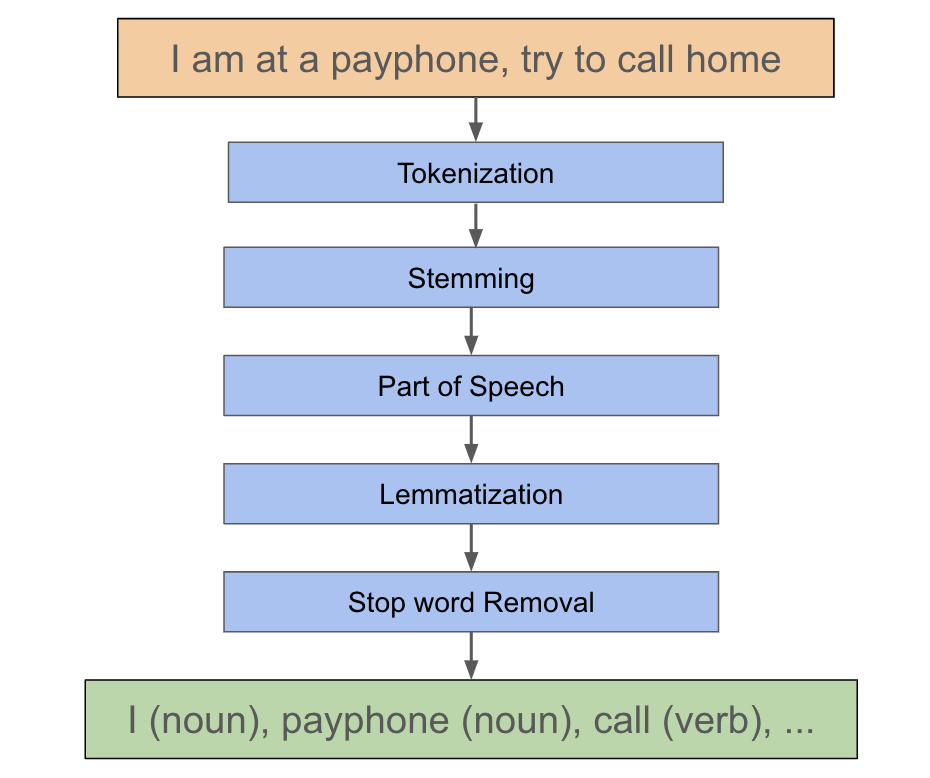
\includegraphics[width=1.0\textwidth]{books/artificial-neural-network/chapter04/figure/pre_processing.png}
	\caption{Luồng tiền xử lý}
	\label{fig:nlp-classic}
\end{center}
\end{figure}

Các bước của Preprocessing thường tùy thuộc vào từng dự án và mục đích. Hình \ref{fig:nlp-classic} mô tả các bước thông dụng trong tiền xử lý. Chi tiết các bước gồm có:
\begin{itemize}
    \item Tiền xử lý chuỗi thô (Bare String Preprocessing): được coi là một trong những bước chính của tiền xử lý. Đây là hành động sử dụng các hàm cụ thể của ngôn ngữ lập trình để sửa đổi dữ liệu đầu vào (như thay thế ký tự, tìm và thay thế các mẫu tự).
    \item Tách từ (Tokenization): là quá trình chuyển một dãy các ký tự thành một dãy các token (token là một dãy các ký tự mang ý nghĩa cụ thể, biểu thị cho một đơn vị ngữ nghĩa trong xử lý ngôn ngữ). Nhiều khi token được hiểu là một từ mặc dù cách hiểu này không hoàn toàn chính xác. Ví dụ như trong tiếng Anh các từ thường được phân tách bằng dấu cách, tuy nhiên từ New York vẫn chỉ được coi là một từ mặc dù nó có dấu cách ở giữa. Do đó chỉ có 1 token trong trường hợp này. Một ví dụ khác là I’m được coi là 2 từ ‘I’ và ‘am’ mặc dù không có dấu cách nào. Trong trường hợp này ta có 2 token. Một điểm cần lưu ý ở đây là chúng ta cần phân biệt khái niệm ‘word type’ và ‘word token’. Types là tổng số các từ có mặt trong một corpus, không tính số lần xuất hiện của từ đó (dù một từ có xuất hiện 40 lần trong đoạn dữ liệu thì cũng chỉ được tính là 1). Trong khi đó, Token tính cả tổng số lần xuất hiện của từng từ. Ví dụ trong câu ‘a good person is a person who is willing to help others’ có tất cả 9 Types (do có 9 từ xuất hiện) nhưng có tới 12 Tokens (do từ ‘a’, ‘person’ và ‘is’ đều xuất hiện 2 lần).
    \item Biến đổi từ về dạng gốc (Stemming): đây là kỹ thuật dùng để biến đổi 1 từ về dạng gốc (được gọi là stem hoặc root form) bằng cách cực kỳ đơn giản là loại bỏ 1 số ký tự nằm ở cuối từ mà nó nghĩ rằng là biến thể của từ. Ví dụ như chúng ta thấy các từ như walked, walking, walks chỉ khác nhau là ở những ký tự cuối cùng, bằng cách bỏ đi các hậu tố -ed, -ing hoặc -s, chúng ta sẽ được từ nguyên gốc là walk.
    \item Phân loại từ trong câu (Part of Speech - POS): POS là việc phân loại các từ trong một câu (danh từ, trạng từ, tính từ hay động từ,...). Việc phân loại từ như thế này sẽ góp phần nắm được thêm ý nghĩa của câu thay vì chỉ xem nó như là tập hợp của các ký tự. Ví dụ như cùng là một từ “can” nhưng nó có thể có nghĩa là “có thể” hoặc nghĩa là “cái lon“, như vậy POS có thể giúp máy tính phân biệt được điều này một cách dễ dàng tùy vào nội dung của câu.
    \item Từ vựng hóa (Lemmatization): Làm trở lại nguyên dạng ban đầu các từ vựng bị biến đổi thể (inflection) hoặc được kết hợp (conjugatetion). Ví dụ như: biến đổi từ ate -> eat.
    \item Loại bỏ các từ dừng (Stop word Removal): Stop word là những từ xuất hiện nhiều trong ngôn ngữ tự nhiên, tuy nhiên lại không mang nhiều ý nghĩa. Trong tiếng Việt, stop word là những từ như: để, này, kia... Tiếng Anh là những từ như: is, that, this... Mục đích của tác vụ này là loại bỏ những từ không mang lại nhiều ý nghĩa cho mô hình.
\end{itemize}

\subsection{Mô hình hóa}
Sau khi thực hiện bứơc tiền xử lý, ta sẽ thực hiện mô hình hóa. Mô hình hóa gồm các bước như sau để thu được output.

\begin{itemize}
    \item Rút trích đặt trưng (Extract features): Để sử dụng được các giải thuật Machine learning, ta cần vector hóa dữ liệu đầu vào. Bước này sẽ giúp ta thực hiện được điều đó.
    \item Xây dựng mô hình (Modelling): dựa vào mục đích ta sẽ xây dựng mô hình, mô hình sẽ còn tuỳ thuộc vào giải thuật Machine learning cụ thể.
    \item Inference: dùng mô hình xây dựng được để áp dụng vào các tác vụ cụ thể.
\end{itemize}

\section{Trích xuất đặc trưng - Feature Extraction}
Trong bước Modeling, trích xuất đặc trưng là một vấn đề khá quan trọng để rút trích các features để đưa vào các model ML.

Dưới đây là 2 phương pháp cơ bản để trích xuất feature:
\begin{itemize}
    \item Vector hóa bằng kỹ thuật đếm (Count-Vectorization - (Bag-of-words) - BOW)
    \item TF-IDF (Term Frequency, Inverse Term Frequency.)
\end{itemize}

\subsection{Phương pháp Bag of words}
Một trong những cách tốt để chuyển các  token thành các feature, cũng là phương pháp mang ý tưởng cốt lõi cho các phương pháp chuyển các  token thành các feature về sau là kỹ thuật BOW. Hướng tiếp cận này rất đơn giản và linh hoạt

Trong phương pháp này, ta sẽ dựa trên những token để tìm tần suất xuất hiện của mỗi token.

Cùng xem ví dụ về 3 câu sau:
\begin{enumerate}
    \item "Hôm qua tôi đi học"
    \item "Hôm nay tôi cũng đi học"
    \item "Ngày mai tôi không đi học"
\end{enumerate}
Thông qua bước tokenization ta biến đổi được thành các câu:
\begin{enumerate}
    \item "Hôm\_qua tôi đi học"
    \item "Hôm\_nay tôi cũng đi học"
    \item "Ngày\_mai tôi không đi học"
\end{enumerate}

Qua bước này "hôm qua", "hôm nay", "ngày mai" được biến đổi thành từ "hôm\_qua", "hôm\_nay", "ngày\_mai".

Ta sẽ xem mỗi câu là một văn bản riêng biệt và ta xây dựng một danh sách tất cả các từ từ 3 câu trên. Ta sẽ được các từ như sau:
\begin{itemize}
    \item Hôm\_qua
    \item Hôm\_nay
    \item Ngày\_mai
    \item tôi
    \item cũng
    \item không
    \item đi
    \item học
\end{itemize}

Bước tiếp theo ta sẽ xây dựng vector. Vector sẽ chuyển các văn bản thành input cho các giải thuật học máy.

Với câu đầu tiên "Hôm\_qua tôi đi học", dựa vào tần suất xuất hiện từ(các từ này là duy nhất trong tập) trong câu ta xây dựng được vector như sau:
\begin{itemize}
   \item 'Hôm\_qua'= 1
    \item 'Hôm\_nay' = 0
    \item 'Ngày\_mai' = 0
    \item 'tôi' = 1
    \item 'cũng' = 0
    \item 'không' = 0
    \item 'đi' = 1
    \item 'học' = 1
\end{itemize}

=> [1, 0, 0, 1, 0, 0, 1, 1]

Các câu còn lại ta sinh được vector như sau:
\begin{itemize}
    \item Hôm\_nay tôi cũng đi học => [0, 1, 0, 1, 1, 0, 1, 1]
    \item Ngày\_mai tôi không đi học => [0, 0, 1, 1, 0, 1, 1, 1]
\end{itemize}

Dưới đây là ma trận ta thu được từ phương pháp BOW (Bảng \ref{tab:bow_vector}):

\begin{table}[h!]
\centering
\begin{tabular}{|l|l|l|l|l|l|l|l|l|}
\hline
Câu & Hôm\_qua & Hôm\_nay   & Ngày\_mai & tôi    & cũng   & không   & đi   & học \\ \hline
Câu 1     & 1     & 0 & 0  & 1    & 0    & 0 & 1 & 1 \\ \hline
Câu 2     & 0     & 1    & 0  & 1 & 1 & 0    & 1    & 1    \\ \hline
Câu 3     & 0     & 0 & 1     & 1 & 0 & 1    & 1    & 1   \\ \hline
\end{tabular}
\caption{Bảng ma trận vector thu được từ phương pháp BOW}
\label{tab:bow_vector}
\end{table}
% \newpage

% Tuy nhiên với phương pháp này, nó tồn tại một số vấn đề bất lợi:

% Đầu tiên là thứ tự các token không được giữ nguyên, điều này ảnh hưởng đến ngữ nghĩa của câu. Đó là lý do tại sao ta gọi là BOW bởi Bag là không mang ý nghĩa thứ tự.

% Thứ hai, bộ đếm không được chuẩn hóa giữa các document với nhau.

\subsection{Phương pháp TF-IDF}

% Thực tế, cách tốt nhất để duy trì các token là việc quan tâm đến các cặp token, bộ ba các token liên tiếp hoặc nhiều hơn thế nữa thay vì chỉ quan tâm đến token riêng lẻ. Cách tiếp cận này được gọi là Extracting-N-Grams. Ví dụ như 1-gram tương ứng với 1 token, 2-gram tuong ứng 2 token, n-gram tương ứng n token.

% Ví dụ sau sẽ minh họa cho bigrams ( 2 cặp token):
% Ta có câu sau "Cause she doesn't get your humor like I do.". Bigrams từ câu này gồm có:

% \begin{itemize}
%     \item 'cause she'
%     \item 'she doesn't'
%     \item 'doesn't get'
%     \item 'get your'
%     \item 'your humor'
%     \item 'humor like'
%     \item 'like I'
%     \item 'I do'
% \end{itemize}

% \begin{figure}[h!]
% \begin{center}
% 	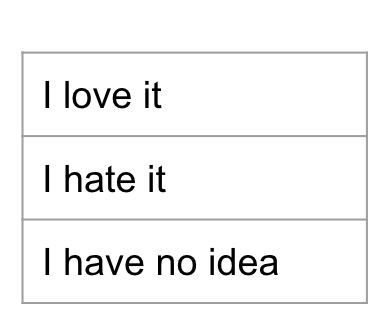
\includegraphics[width=0.25\textwidth]{books/artificial-neural-network/chapter04/figure/example.png}
% 	\caption{Ví dụ minh họa TF-IDF}
% 	\label{fig:nlp-classic}
% \end{center}
% \end{figure}

% Với cùng 3 ví dụ ở mục trước, bây giờ các cột ko phải chỉ là 1 token riêng biệt mà bây giờ là một cặp token. Và các câu review cũng được chuyển sang dạng vector một cách tương ứng với phương pháp Bag of words, với giá trị 1 / 0 thể hiện cho việc cặp token có xuất hiện / ko xuất hiện trong câu review tương ứng hay không.

% Hãy để ý ở đây, cách biểu diễn ở mức này mới chỉ đưa ra được mối quan hệ thứ tự cục bộ (local) trong câu, nhưng cái mà ta mong muốn là phân tích đoạn text đầu vào một cách tốt hơn. Và một vấn đề nữa đó là sẽ có rất nhiều các feature mà ta sẽ có ở đây nếu lấy một cặp các token. Giả sử số lượng token lên đến 100000 token thì số lượng các features có thể tăng lên theo cấp số mũ.

% Để giải quyết vấn đề này, ta sẽ loại bỏ một số n-grams dựa trên tần suất xuất hiện của chúng trong tập hợp các câu review đầu vào của ta (corpus). Có ba trường hợp gồm:
% \begin{itemize}
%     \item n-grams có tần suất xuất hiện cao
%     \item n-grams có tần suất xuất hiện thấp
%     \item n-grams có tần suất xuất hiện trung bình
% \end{itemize}


% n-grams có tần suất xuất hiện cao: trường hợp này xuất hiện trong hầu hết các văn bản, bạn đều có thể thấy được n-grams này. Ví dụ với Tiếng Anh, đó có thể là các giới từ (a, an, this, that, v.v... ). Và bởi vì ta chỉ sử dụng cấu trúc ngữ pháp, cho nên chúng không có ý nghĩa nhiều lắm. Chúng được gọi với cái tên là stop words, nó không thực sự giúp ta phân biệt các đoạn text với nhau, nên các từ này này cần được loại bỏ.

% n-grams có tần suất xuất hiện thấp: trường hợp này đến từ lỗi gõ sai từ người dùng, hoặc là thường hiếm xuất hiện trong bất kỳ các văn bản nào trong tập dữ liệu của  ta. Các trường hợp này cũng cần nên loại bỏ vì nó sẽ gây ra overfit cho model.

% n-grams có tần suất xuất hiện trung bình: đây là các n-grams tốt nhất bởi vì chúng bao gồm n-grams mà không có 2 trường hợp nêu trên. Vấn đề là trong tập n-grams có tấn suất xuất hiện trung bình, có rất nhiều n-grams thuộc các dải tần số xuất hiện khác nhau. Thật hữu ích khi chúng hữu dụng để có thể dựa vào tần số mà có thể lọc được n-grams là tốt, n-grams nào là xấu hơn. Nếu  ta có thể ranking các n-grams này theo mức độ quan trọng của chúng thì sẽ ra sao, chắc chắn sẽ rất có lợi. Chúng ta có thể quyết định được n-grams với tần suất xuất hiện trung bình thì n-grams nào là tốt, n-grams nào là xấu. Và ý tưởng ở đây là : n-grams có tần suất nhỏ hơn sẽ được đánh trọng số cao hơn vì nó là thể hiện cho các trường hợp riêng biệt trong câu review.



TF-IDF là từ viết tắt của thuật ngữ tiếng Anh "term frequency – inverse document frequency", TF-IDF là trọng số của một từ trong văn bản thu được qua thống kê thể hiện mức độ quan trọng của từ này trong một văn bản, mà bản thân văn bản đang xét nằm trong một tập hợp các văn bản. TF-IDF khắc phục được nhược điểm của BOW.

Ví dụ ta có một câu như sau:

"Today is a beautiful day"

Bạn nghĩ gì khi đọc câu này? Từ gì bạn tập trung nhiều hơn. Câu này nói về hôm nay (today), nó cũng nói là hôm nay là ngày đẹp trời (today is a beautiful day), cảm xúc trong câu này là tích cực, vui vẻ. Đẹp (beauty) rõ ràng là tính từ được sử dụng ở đây. Với phương pháp BOW, tất cả các từ đều có cùng số lần xuất hiện (tần suất) như nhau (1 trong trường hợp này) và rõ ràng các từ đều được coi ngang hàng nhau (tầm quan trọng như nhau (và không nhấn mạnh được từ cần nhấn mạnh trong câu (từ beauty).

Một trường hợp khác, trong một tài liệu có 200 từ, từ 'a', 'the' xuất hiện rất nhiều lần (20 lần từ 'a', 15 lần từ 'the'). Những từ này xuất hiện nhiều lần không có nghĩa là chúng quan trọng. BOW cũng không giải quyết được vấn đề này.

Ưu điểm:
\begin{itemize}
    \item Dễ tính toán
    \item Đây là cách đon giản để trích xuất các mô tả trong văn bản
    \item Dễ dàng tính toán sự giống nhau giữa 2 văn bản
\end{itemize}

Nhược điểm:
\begin{itemize}
    \item TF-IDF dựa trên BOW nên vì thế nó không thể thể hiện tầm quan trọng của vị trí từ trong văn bản, ngữ nghĩa, sự tương quan giữa các từ trong các văn bản khác nhau
\end{itemize}

TF-IDF gồm 2 trọng số TF và IDF.

TF - Term Frequency : dùng để ước lượng tần xuất xuất hiện của từ trong văn bản. Tuy nhiên với mỗi văn bản thì có độ dài khác nhau, vì thế số lần xuất hiện của từ có thể nhiều hơn. Vì vậy số lần xuất hiện của từ sẽ được chia độ dài của văn bản (tổng số từ trong văn bản đó)

\begin{center}
    $TF(t, d) =  \frac{( \text{số lần từ t xuất hiện trong văn bản d})}{ (\text{tổng số từ trong văn bản d})}$
\end{center}

IDF - Inverse Document Frequency: dùng để ước lượng mức độ quan trọng của từ đó như thế nào . Khi tính tần số xuất hiện TF thì các từ đều được coi là quan trọng như nhau. Tuy nhiên có một số từ thường được được sử dụng nhiều nhưng không quan trọng để thể hiện ý nghĩa của đoạn văn, ví dụ:
\begin{itemize}
    \item Từ nối: và, nhưng, tuy nhiên, vì thế, vì vậy,...
    \item Giới từ: ở, trong, trên,...
    \item Từ chỉ định: ấy, đó, nhỉ,...
\end{itemize}

Vì vậy ta cần giảm đi mức độ quan trọng của những từ đó bằng cách sử dụng IDF

\begin{center}
    \(IDF(t, D) = log(\frac{\text{Tổng số văn bản trong tập mẫu D}}{\text{Số văn bản có chứa từ t}})\)
\end{center}

Từ đó ta có công thức TF-IDF

\begin{center}
    \(TFIDF(t, d, D) = TF(t, d) x IDF(t, D)\)
\end{center}

Mỗi tài liệu sẽ được biểu diễn bằng một vector tf.idf, vector này sẽ số chiều là K với K độ dài tất cả các từ có trong tất cả các văn bản của tập dữ liệu.

Ví dụ về TF-IDF:

Dữ liệu ban đầu ta có 3 văn bản như sau:
\begin{itemize}
    \item Document 1: "Hôm\_qua tôi đi học"
    \item Document 2: "Hôm\_nay tôi cũng đi học"
    \item Document 3: "Ngày\_mai tôi không đi học"
\end{itemize}

Đầu tiên ta sẽ xây dựng bảng từ vựng trong corpus. Bảng \ref{tab:sec3exmptfidf} là bảng ta thu được khi xây dựng bảng từ vựng.
\begin{table}[h!]
\centering
\begin{tabular}{|l|l|lll}
\cline{1-2}
Word  & Count &  &  &  \\ \cline{1-2}
Hôm\_qua & 1     &  &  &  \\ \cline{1-2}
Hôm\_nay    & 1     &  &  &  \\ \cline{1-2}
Ngày\_mai & 1     &  &  &  \\ \cline{1-2}
tôi & 3     &  &  &  \\ \cline{1-2}
cũng & 1     &  &  &  \\ \cline{1-2}
không & 1     &  &  &  \\ \cline{1-2}
đi & 3     &  &  &  \\ \cline{1-2}
học & 3     &  &  &  \\ \cline{1-2}
\end{tabular}
\caption{Bảng từ vừng trong corpus}
\label{tab:sec3exmptfidf}
\end{table}

Tiếp theo ta sẽ tính TF cho mỗi từ ứng với mỗi văn bản trong corpus. Bảng \ref{tab:sec3caltf} là kết quả tính giá trị TF cho mỗi từ vựng ứng với mỗi văn bản.

\begin{table}[h!]
\centering
\begin{tabular}{|l|l|l|l|l}
\cline{1-4}
Words/Document & Document 1 & Document 2 & Document 3 &  \\ \cline{1-4}
Hôm\_qua          & 0.25       & 0       & 0       &  \\ \cline{1-4}
Hôm\_nay          & 0       & 0.2          & 0       &  \\ \cline{1-4}
Ngày\_mai          & 0       & 0       & 0.2          &  \\ \cline{1-4}
tôi              & 0.25          & 0.2       & 0.2       &  \\ \cline{1-4}
cũng             & 0          & 0.2       &  0      &  \\ \cline{1-4}
không             & 0       & 0          & 0.2          &  \\ \cline{1-4}
đi             & 0.25       & 0.2          & 0.2          &  \\ \cline{1-4}
học           & 0.25       & 0.2          & 0.2          &  \\ \cline{1-4}
\end{tabular}
\caption{Bảng tính TF cho các tài liệu}
\label{tab:sec3caltf}
\end{table}

Bước kế tiếp ta cần tính giá trọ IDF cho mỗi từ vựng. Bảng \ref{tab:sec3calidf} liệt kê kết quả tính IDF cho mỗi từ vựng.

\begin{table}[h!]
\centering
\begin{tabular}{|l|l|l}
\cline{1-2}
Words & IDF value &  \\ \cline{1-2}
Hôm\_qua & log(3/1) = 0.48 &  \\ \cline{1-2}
Hôm\_nay    & log(3/1) = 0.48 &  \\ \cline{1-2}
Ngày\_mai & log(3/1) = 0.48 &  \\ \cline{1-2}
tôi     & log(3/3) = 0  &  \\ \cline{1-2}
cũng    & log(3/1) = 0.48 &  \\ \cline{1-2}
không    & log(3/1) = 0.48 &  \\ \cline{1-2}
đi    & log(3/3) = 0 &  \\ \cline{1-2}
học  & log(3/3) = 0 &  \\ \cline{1-2}
\end{tabular}
\caption{Bảng tính IDF cho các văn bản}
\label{tab:sec3calidf}
\end{table}

Cuối cùng ta dựa vào giá trị TF và IDF ta sẽ tính được vector TF-IDF cho mỗi từ vựng dựa theo công thức \(TF-IDF = TF . IDF\). Bảng \ref{tab:sec3caltfidf} mô tả ma trận kết quả thu được.

\begin{table}[h!]
\centering
\begin{tabular}{|l|l|l|l|l|l|l|l|l|}
\hline
  & Hôm\_qua & Hôm\_nay & Ngày\_mai & tôi    & cũng   & không   & đi  & học \\ \hline
Document 1     & 0.12     & 0 & 0  & 0    & 0    & 0 & 0 & 0 \\ \hline
Document 2     & 0     & 0.1    & 0  & 0 & 0.1 & 0    & 0    & 0    \\ \hline
Document 3     & 0     & 0 & 0.1     & 0 & 0 & 0.1    & 0    & 0    \\ \hline
\end{tabular}
\caption{Bảng tính TF-IDF}
\label{tab:sec3caltfidf}
\end{table}
\newpage

Sau khi tính TF-IDF, mỗi document đã được vector hóa bằng phương pháp này (số chiều của vector chính là số từ ta trong tất cả document, số chiều = 8) gồm:

\begin{itemize}
    \item "Hôm\_qua tôi đi học" =>  [0,12, 0, 0,0, 0, 0, 0, 0]
    \item  "Hôm\_nay tôi cũng đi học" => [0, 0.1, 0, 0, 0.1, 0, 0, 0]
    \item "Ngày\_mai tôi không đi học" [0, 0, 0.1, 0, 0, 0.1, 0, 0]
\end{itemize}

Dựa vào công thức TF-IDF ta cũng nhận ra một hạn chế của $TF_IDF$ này là không biểu diễn được quan hệ giữa các từ trong văn bản.

Ví dụ như câu: "Đi học hôm\_qua tôi" thông qua TF-IDF cũng ra vector [0,12, 0, 0,0, 0, 0, 0, 0] tương tự câu "Hôm\_qua tôi đi học".

\section{Mô hình xử lý ngôn ngữ tự nhiên bằng mạng học sâu}
Hướng tiếp cận cổ điển của việc xử lý ngôn ngữ tự nhiên (NLP - Natural Language Processing, hình \ref{fig:pipeline-nlp-classic}) đã sử dụng trong nhiều năm trước về căn bản đã có thể thay thế bằng mô hình Deep Learning (gọi tắt là DL). Hình \ref{fig:deep-learning-based-nlp} là một mô hình đơn giản được đưa ra nhằm mục đích để  cố gắng đạt được những kết quả mong đợi như phương pháp tiếp cận cổ điển đã đem đến nhưng với hướng tiếp cận hiện đại - sử dụng mô hình học sâu. Hiện nay, đã có rất nhiều mô hình DL cùng các kĩ thuật phức tạp được đề ra nhằm để giải quyết các bài toán khác nhau, nhưng về căn bản thì mọi thứ đã được thể hiện thông qua hình \ref{fig:deep-learning-based-nlp}.

\begin{figure}[h!]
\begin{center}
	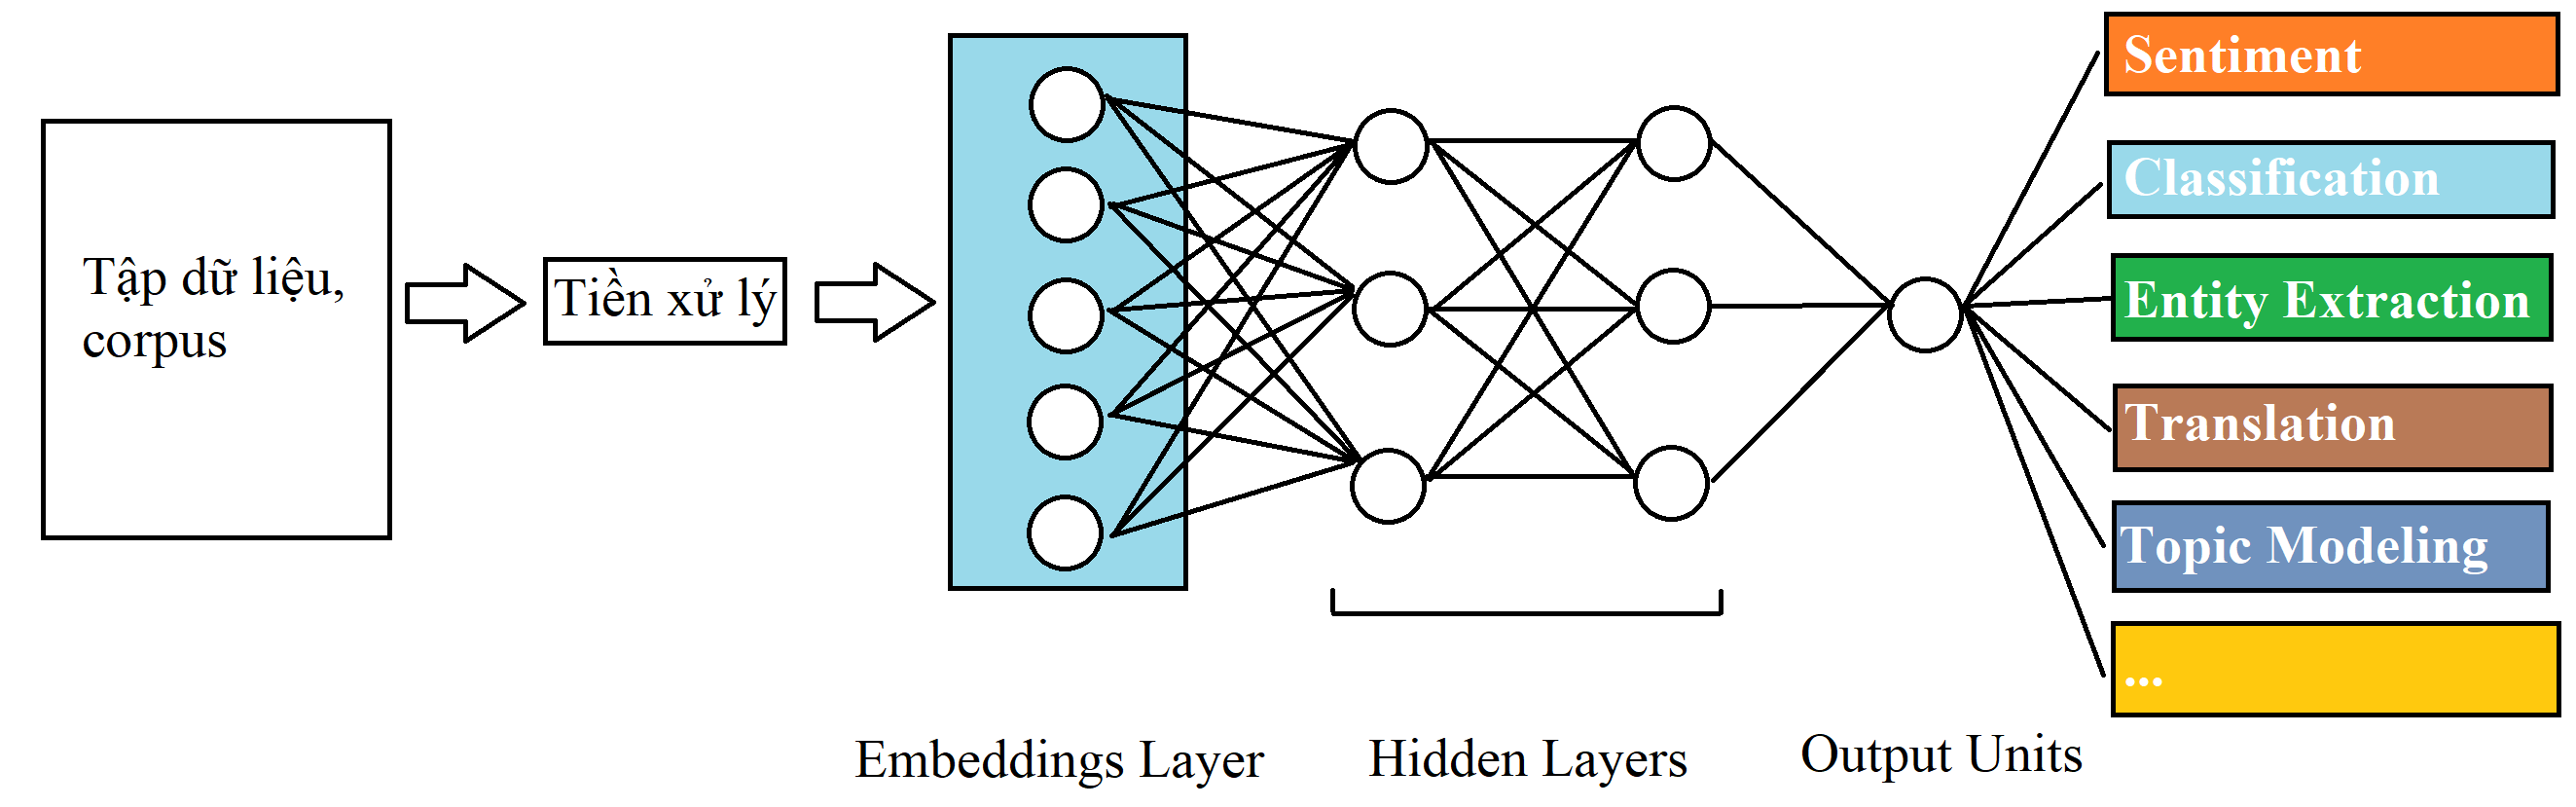
\includegraphics[width=1.0\textwidth]{books/artificial-neural-network/chapter04/figure/nlp-deep-model.png}
	\caption{Mô hình Deep Learning sử dụng cho NLP}
	\label{fig:deep-learning-based-nlp}
\end{center}
\end{figure}

Dựa vào đó, ta có thể thấy rằng, để xây dựng mô hình NLP dựa trên Deep Learning thì ta cần phải trải qua một số bước:
\begin{itemize}
    \item Cũng như mô hình cổ điển, dữ liệu được dùng để huấn luyện cũng cần phải trải qua bước tiền xử lý như tokenization, biến đổi từ về dạng gốc, từ vựng hóa, loại bỏ các từ vựng...
    \item Sau đó, do mạng Deep Learning chỉ tương tác trên các ma trận, vector và con số nên sẽ cần có một bước để chuyển các từ này thành các vector. Đó chính là mục tiêu chính của Embedding Layer.
    \item Và liền kề theo đó thì bước Modeling của mô hình cổ điển cũng sẽ được thay thế bằng kiến trúc hiện đại hơn - Neural Network. Và Output của Neural Network này sẽ được sử dụng phù hợp đối với từng công việc khác nhau như Sentiment, Classification, Topic Modeling...
\end{itemize}

Như vậy khi ta áp dụng mô hình vào một bài toán nhất định, ta có thể thấy là một cách rất tự nhiên rằng sau khi huấn luyện kết thúc, mạng Deep Learning có thể tự động học, sau đó đã rút trích được các đặc trưng cần thiết và biến đổi chúng thành các trọng số  ở các Hidden Layers. Đây cũng chính là lý do giải thích cho ta thấy được rằng kiến trúc mạng Deep Neural Network có thể được sử dụng để thay thế cho mô hình xử lý ngôn ngữ tự nhiên cổ điển.

Quay lại với Embeddings Layer, có rất nhiều cách để có thể biến đổi dữ liệu đầu vào thành các vector. Với 3 tài liệu ở ví dụ đầu tiên đã nêu ra, ta sẽ có một tập từ điển có 8 từ được sắp xếp theo bảng chữ cái. Thì một trong những cách biến đổi là mỗi tài liệu ứng với 1 vector 1 x 8 (do có 8 từ), giá trị của các phần tử trong vector này chính là số lần xuất hiện của từ đó trong tài liệu. Ví dụ, với tài liệu là "Hôm\_qua tôi đi học" sẽ tương đương với vector là [0 1 1 0 1 0 0 1].

Tuy nhiên, nhờ vào sức mạnh tính toán của mạng học sâu, ta vẫn có cách biểu điễn để giúp cho tập tài liệu của ta thể hiện nhiều thông tin hơn. Cụ thể hơn là thay vì biểu diễn cả tài liệu chỉ thông qua một vector thì ta sẽ biểu diễn từng từ trong tài liệu thành từng vector. Điều này có nghĩa với cách tiếp cận này, sau khi ta áp dung cho tập tài liệu "Hôm\_qua tôi đi học" thì ta sẽ tạo ra được một ma trận 4 x 8 (do có 4 từ, mỗi từ được thể hiện bằng một vector có kích thước là 8).

Quá trình biến đổi từ thành các vector này còn được biết đến với một cái tên khác là Word Embedding. Trong mục \ref{sec:word-embedding-in-details}, ta sẽ tìm hiểu kĩ hơn về các kĩ thuật được sử dụng cho Word Embedding một cách chi tiết để sử dụng chúng hiệu quả hơn.